\chapter{Elliptic curves}

\epigraph[author={Serge Lang}, source={Elliptic Curves: Diophantine Analysis}]{It is possible to write endlessly on elliptic curves. (This is not a threat.)}\SubIndex{Lang, Serge}


\section{Cubic curves}

\begin{theorem}[Chasles]\label{theorem:Chasles}\define{theorem!Chasles}\define{Chasles theorem}
Suppose that \(C_1\) and \(C_2\) are plane cubic curves intersecting at 9 points over the algebraic closure of the field.
Every plane cubic curve passing through any \(8\) of those points passes through all \(9\).
The plane cubic curves passing through those \(9\) points are precisely the pencil through \(C_1\) and \(C_2\).
\end{theorem}
\begin{proof}
By theorem~\vref{theorem:independence}, with \(n=8\) and \(d=3\), either 
\begin{enumerate}
\item
\(8\) of the points impose independent conditions or
\item
\(5\) of the points are colinear or
\item
all \(8\) of the points lie on a conic.
\end{enumerate}
If \(7\) of the points lie on a conic, then by B\'ezout's theorem that conic lies in both \(C_1\) and \(C_2\), so \(C_1\) and \(C_2\) have infinitely many points in common, a contradiction.
If \(4\) of the points lie on a line, then by B\'ezout's theorem that line lies in both \(C_1\) and \(C_2\), so \(C_1\) and \(C_2\) have infinitely many points in common, a contradiction.
So all \(8\) points inmpose independent conditions, i.e. the projective space of cubics through all \(8\) points has dimension \(3^*-8=1\).
Since \(C_1 \ne C_2\), the projective space of cubics through all \(9\) points has dimension at least 1: the pencil through \(C_1\) and \(C_2\) is 1-dimensional.
But the family through all \(9\) points is a projective subspace of the family through all \(8\) points.
Both projective spaces have the same dimension, hence these two projective spaces are equal.
\end{proof}


\begin{center}
\documentclass{standalone}
\usepackage{tikz}
\usepackage{pgfplots}
\usepackage{xparse}
\pgfplotsset{compat=1.12,width=7cm}%
\colorlet{curveZero}{gray!85}
\colorlet{curveOne}{blue!60}
\definecolor{curveOneColor}{rgb}{.6,0,0}
\colorlet{curveTwo}{brown!50!gray}
\colorlet{curveThree}{green!40!gray}
\colorlet{curveFour}{red!50!gray}
\NewDocumentCommand\DrawDotInPlot{O{}mmO{}}%
{%
\fill[gray!15,draw=gray] (axis cs:{#2},{#3}) circle [radius=1.6pt] node[above,black,#4] {\(#1\)};%
}%
\NewDocumentCommand\DrawDot{O{}mmO{}}%
{%
\fill[gray!20,draw=gray] ({#2},{#3}) circle (1.6pt) node[above,black,#4] {\(#1\)};%
}%
\NewDocumentCommand\DrawNode{O{}m}%
{%
\fill[gray!20,draw=gray] (#2) circle (1.6pt) node[above,black] {\(#1\)};%
}%
\NewDocumentCommand\DrawDotThreeD{O{}mmmO{}}%
{%
\fill[gray!20,draw=gray] ({#2},{#3},{#4}) circle (1.6pt) node[above,black,#5] {\(#1\)};%
}%
\colorlet{axisColor}{gray!50}
\tikzstyle{shapeZero}=[fill=curveZero,opacity=.4]
\tikzstyle{shapeOne}=[fill=curveOne,opacity=.4]
\tikzstyle{shapeTwo}=[fill=curveTwo,opacity=.4]
\tikzstyle{shapeThree}=[fill=curveThree,opacity=.4]
\tikzstyle{groupElementLabel}=[minimum size=2.4em]
\tikzstyle{groupElement}=[minimum size=2.4em,shapeZero,draw=curveZero]
\tikzstyle{cosetOne}=[minimum size=2.4em,shapeOne,draw=curveOne]
\tikzstyle{cosetTwo}=[minimum size=2.4em,shapeTwo,draw=curveTwo]


\begin{document}
\begin{tikzpicture}
\begin{axis}[hide axis,xmin=-2,xmax=2,ymin=-2,ymax=2]
\newcommand{\RRR}{1.8}
\draw[axisColor] 
	(\RRR,0) 
-- ({-\RRR},0);
  \addplot[very thick,domain=-1:0,curveZero,samples=200]{sqrt((x+1)*x*(x-1))};%
  \addplot[very thick,domain=-1:0,curveZero,samples=200]{-sqrt((x+1)*x*(x-1)))};%
  \addplot[very thick,domain=1:2,curveZero,samples=200]{sqrt((x+1)*x*(x-1)))};%
  \addplot[very thick,domain=1:2,curveZero,samples=200]{-sqrt((x+1)*x*(x-1)))};%
\DrawDotInPlot{0}{0}
\DrawDotInPlot{1}{0}
\DrawDotInPlot{-1}{0}
\end{axis}
\end{tikzpicture}
\end{document}

\end{center}
For any two distinct points \(p, q\) of a cubic curve \(C\), the line through \(p\) and \(q\) intersects \(C\) in three points; let \(r\) be the third point.
If \(p\) and \(q\) are defined in some field \(k\), then so is the line through \(p\) and \(q\).
Suppose that \(C\) is also defined over \(k\).
On that line, parameterized over \(k\) as \(y=mx+b\), the cubic equation of \(C\) (having coefficients over \(k\)) restricts to have at least two roots in \(k\), corresponding to the points \(p\) and \(q\).
So that cubic polynomial on the line factors into linear factors over \(k\).
That third root gives the location of \(r\) on that line: the point \(r\) is also defined over \(k\).

We can extend this definition to allow \(p=q\), by taking \(r\) to be the point of \(C\) at which the tangent line to \(\ell\) to \(C\) at \(p\) touches \(C\) again. 
\begin{center}
\documentclass{standalone}
\usepackage{tikz}
\usepackage{pgfplots}
\pgfplotsset{compat=1.12,width=7cm}%
\usepackage{xparse}
\colorlet{curveZero}{gray!85}
\colorlet{curveOne}{blue!60}
\definecolor{curveOneColor}{rgb}{.6,0,0}
\colorlet{curveTwo}{brown!50!gray}
\colorlet{curveThree}{green!40!gray}
\colorlet{curveFour}{red!50!gray}
\NewDocumentCommand\DrawDotInPlot{O{}mmO{}}%
{%
\fill[gray!15,draw=gray] (axis cs:{#2},{#3}) circle [radius=1.6pt] node[above,black,#4] {\(#1\)};%
}%
\NewDocumentCommand\DrawDot{O{}mmO{}}%
{%
\fill[gray!20,draw=gray] ({#2},{#3}) circle (1.6pt) node[above,black,#4] {\(#1\)};%
}%
\NewDocumentCommand\DrawNode{O{}m}%
{%
\fill[gray!20,draw=gray] (#2) circle (1.6pt) node[above,black] {\(#1\)};%
}%
\NewDocumentCommand\DrawDotThreeD{O{}mmmO{}}%
{%
\fill[gray!20,draw=gray] ({#2},{#3},{#4}) circle (1.6pt) node[above,black,#5] {\(#1\)};%
}%
\colorlet{axisColor}{gray!50}
\tikzstyle{shapeZero}=[fill=curveZero,opacity=.4]
\tikzstyle{shapeOne}=[fill=curveOne,opacity=.4]
\tikzstyle{shapeTwo}=[fill=curveTwo,opacity=.4]
\tikzstyle{shapeThree}=[fill=curveThree,opacity=.4]
\tikzstyle{groupElementLabel}=[minimum size=2.4em]
\tikzstyle{groupElement}=[minimum size=2.4em,shapeZero,draw=curveZero]
\tikzstyle{cosetOne}=[minimum size=2.4em,shapeOne,draw=curveOne]
\tikzstyle{cosetTwo}=[minimum size=2.4em,shapeTwo,draw=curveTwo]


\begin{document}
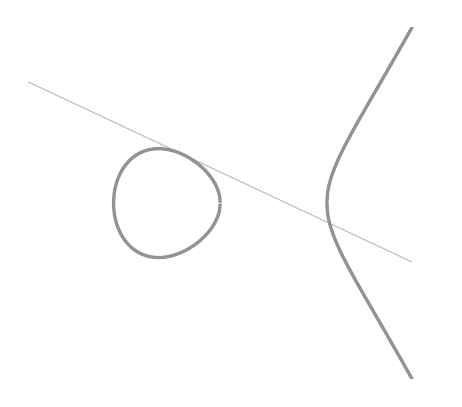
\begin{tikzpicture}
\begin{axis}[hide axis,xmin=-2,xmax=2,ymin=-2,ymax=2]
\newcommand{\fn}[1]{sqrt((#1+1)*(#1)*(#1-1))}
\newcommand{\xnought}{-.35}
\pgfmathsetmacro{\ynought}{0.554188596057335}
\pgfmathsetmacro{\slope}{-0.570654109900308}
\newcommand{\xone}{-1.8}
\pgfmathsetmacro{\yone}{1.38163705541278}
\newcommand{\xtwo}{1.8}
\pgfmathsetmacro{\ytwo}{-0.672717740228328}
\draw[axisColor] 	(axis cs:{\xone},{\yone}) -- (axis cs:{\xtwo},{\ytwo});
  \addplot[very thick,domain=-1:0,curveZero,samples=200]{sqrt((x+1)*x*(x-1))};%
  \addplot[very thick,domain=-1:0,curveZero,samples=200]{-sqrt((x+1)*x*(x-1)))};%
  \addplot[very thick,domain=1:2,curveZero,samples=200]{sqrt((x+1)*x*(x-1)))};%
  \addplot[very thick,domain=1:2,curveZero,samples=200]{-sqrt((x+1)*x*(x-1)))};%
  \DrawDotInPlot[p]{\xnought}{\ynought}
  \DrawDotInPlot[r]{1.02564611314611}{-0.230829512177879}[below left]
\end{axis}
\end{tikzpicture}
\end{document}

\end{center}

With a little algebra by hand, and some sage code to solve the mess, we can find the intersection points of tangent lines.
Consider the curve
\[
C=(y^2-(x+1)x(x-1))
\] 
and the point \(p\) with \(p=(x,y)\) with \(x=-35/100\):
\begin{sageblock}
X=-35/100
Y=sqrt((X+1)*X*(X-1))
# The slope of the tangent line is given by implicit differentation.
M=(3*X^2-1)/(2*Y)
# Write the equation of the curve restricted to the tangent line.
x=var('x')
f=(Y+M*(x-X))^2-(x+1)*x*(x-1)
print("The tangent line strikes the curve at ",solve(f,x))
XX=(201601/196560)
YY=-sqrt((XX+1)*XX*(XX-1))
print("The other intersection point is ",XX.n(),YY.n())
plot(f,x,-2,2)
\end{sageblock}

\section{Elliptic curves}
A \emph{elliptic curve}\define{elliptic curve}\define{curve!elliptic} over a field \(k\) is a smooth plane cubic curve \(C\) defined over \(k\) with a chosen point \(o\) of \(C\), also defined over \(k\), which we think of as the ``origin'' of \(C\).
Given any point \(p\) of \(C\), the line \(op\) contains three points of \(C\) (counting with multiplicity if needed), say \(p,o,\bar{p}\).
Define the \emph{addition} of points \(p,q\) by taking the line \(pq\), which then intersects \(C\) at \(3\) points, say \(p,q,r\), and then defining \(p+q\) to be \(\bar{r}\), so \(p+q,r,o\) are the three points at which a line intersects \(C\).
Danger: note that this addition is \emph{not} the same as adding the coordinates of the points, as you would do in linear algebra.

What if \(p=q\)?
The tangent line to \(C\) at \(p\) intersects \(C\) at some point not equal to \(p\), say \(r\), and define \(p+p=\bar{r}\).

\begin{theorem}
Any elliptic curve is an abelian group under the addition operation.
\end{theorem}
\begin{proof}
If \(p,q,r\) are the points at which a line intersects a cubic \(C\), then so are \(q,p,r\), and so \(p+q=\bar{r}=q+p\).
By definition, \(p,o,\bar{p}\) are on a line, so \(\bar{\bar{p}}=p\) and so \(p+o=\bar{\bar{p}}=p\).

Consider the point \(\bar{o}\), i.e. so that the line \(\bar{o}o\) is the tangent line to \(C\) at \(o\).
Let \(-p=\overline{p+\bar{o}}\), i.e. \(-p,p,\bar{o}\) are on a line.
So then \(p+(-p)=\bar{\bar{o}}=o\).

Any equation like \(r+q=p+q\) forces the points \(r,q,\overline{r+q}\) to be \(r,q,\overline{p+q}\), and hence to be \(p,q,\overline{p+q}\), so \(p=r\), we can cancel.

By definition of addition, for any two points \(p,q\) of \(C\),
\[
p,\overline{p+q},\overline{p+\overline{p+q}}
\]
lie in a line, while 
\[
p,q,\overline{p+q}
\]
do as well, so 
\[
q=\overline{p+\overline{p+q}},
\]
i.e.
\[
\bar{q}=p+\overline{p+q},
\]
a ``funny cancellation''.

Take three points \(p,q,r\) of \(C\).
We want to prove that \(p+(q+r)=(p+q)+r\).
Suppose that \(p=o\) or \(q=o\) or \(r=o\) or \(p=r\).
The equation \(p+(q+r)=(p+q)+r\) follows from any of these.
So we can suppose that none of these is satisfied.

Define lines
\begin{align*}
L_1 &= p(q+r), \\
L_2 &= rq, \\
L_3 &= o(p+q), \\
L'_1 &= r(p+q), \\
L'_2 &= pq, \\
L'_3 &= o(r+q).
\end{align*}

Note that \(p,q+r\) lie on \(L_1\), and so therefore does \(\overline{p+(q+r)}\).
Similarly,
\begin{align*}
p,q+r,\overline{p+(q+r)} & \in L_1, \\
r,q,\overline{q+r} & \in L_2, \\
o,p+q,\overline{p+q} & \in L_3, \\
r,p+q,\overline{(p+q)+r} & \in L'_1, \\
p,q,\overline{p+q} & \in L'_2, \\
o,q+r,\overline{q+r} & \in L'_3.
\end{align*}

Suppose that \(L_1 = L_1'\).
So the points \(p,q+r,\overline{p+(q+r)}\) are some permutation of the points \(r,p+q,\overline{(p+q)+r}\).
This forces \(p=r\) or \(p=p+q\) or \(q+r=r\) or \(q+r=p+q\), and after cancellation these becomes \(p=r\) or \(q=o\), contradicting our hypotheses.

So \(L_1 \ne L_1'\).
Take the point \(s\) where \(L_1\) and \(L_1'\) intersect.
If \(s\) lies on \(C\), then \(s\) lies on \(p,q+r,s\), so \(\bar{s}=p+(q+r)\), but also \(s\) lies on \(r,p+q,s\), so \(\bar{s}=(p+q)+r\).
So \(s\) lies on \(C\) just when \(p+(q+r)=(p+q)+r\).

Consider the \(8\) points \(o,p,q,r,q+r,p+q,\) and a ninth point \(s\).
The cubic \(L_1 \cup L_2 \cup L_3\) contains all \(9\) points, as does the cubic \(L_1' \cup L_2' \cup L_3'\).
Suppose that these cubics have no component in common.
Then by Chasles's theorem (theorem~\vref{theorem:Chasles}), the plane cubics containing the \(8\) points contain all \(9\), so \(s\) belongs to \(C\).

Suppose that these cubics share a component, say \(L_i = L_j'\).
The 3 points of \(C\) on \(L_i\) and the \(3\) points on \(L_j'\) must be the same \(3\) points.
No other point of the cubic \(C\) can lie on that line, by B\'ezout's theorem.
So the remaining \(5\) points lie on the other lines.
Each pair of remaining lines is a conic.
By lemma~\vref{lemma:conics.5.points}, these conics are equal or share a common line through \(4\) of the points.
But we can't have \(4\) points of \(C\) on the same line, by B\'ezout's theorem.
So these conics are equal, i.e. all three lines \(L_1,L_2,L_3\) are the same as \(L_1',L_2',L_3'\) up to reordering.

We know that \(L_1 \ne L_1'\), so \(L_1=L_2'\) or \(L_1=L_3'\).
Swapping \(p\) and \(r\) swaps primed and unprimed lines.

If \(L_2=L_2'\), the points \(r,q,\overline{q+r}\) are the same as \(p,q,\overline{p+q}\), up to reordering.
If this forces \(r=p\), we have seen that \(p+(q+r)=(p+q)+r\) follows.
Otherwise, we find \(\overline{q+r}=p\) and \(r=\overline{p+q}\), and then
\[
p+(q+r)=p+\bar{p}=\bar{o},
\]
and
\[
(p+q)+r=\bar{r}+r=\bar{o}.
\]
So we can assume that \(L_2 \ne L_2'\).

If \(L_3=L_3'\), the points \(o,p+q,\overline{p+q}\) are the same as \(o,r+q,\overline{r+q}\).
Since we suppose that \(p \ne r\), \(r+q=\overline{p+q}\).
By funny cancellation,
\[
p+(q+r)=p+\overline{p+q}=\bar{q},
\]
while
\[
(p+q)+r=\overline{q+r}+r=r+\overline{r+q}=\bar{q},
\]
so again \(p+(q+r)=(p+q)+r\).

If \(L_2=L_3'\) then \(r=o\) or \(q=o\), a contradiction.

Hence \(L_1, L_2, L_3\) must be some permutation of \(L_1',L_2',L_3'\), but we can't have \(L_1=L_1'\) or \(L_2=L_2'\) or \(L_2=L_3'\) or \(L_3=L_3'\).
So \(L_1=L_3'\).
Permutation of \(p\) and \(r\) then forces \(L_3=L_1'\), so \(L_2=L_3'\), a contradiction.
\end{proof}



\begin{example}
We always take an elliptic curve to be a smooth cubic \(C\) with a chosen point \(o \in C\), giving an addition operation as above.
If we pick some other point \(o'\) of our cubic curve \(C\) to be the ``origin'' of an elliptic curve, then we get another addition operation, say \(+'\).
The map
\[
p \in C \mapsto p+(o'-o),
\]
using the operations defined above is an isomorphism of groups from \(C\) with \(+\) to \(C\) with \(+'\).
So the choice of point \(o\) is not very important.
\end{example}
